La Núria té un jardí rectangular i vol fer-hi un tancat (rectangular o quadrat) de $8\ \text{m}^2$ per al seu gos. Ha pensat
de posar el tancat tocant al mur del jardí, tal com es mostra a la figura, per estalviar-se així un dels quatre costats.
El preu de la tanca que vol fer servir és de 2,5 €/m.
\begin{center}
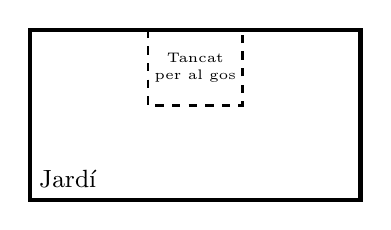
\begin{tikzpicture}[scale=0.6]
  \draw[line width=1.6pt] (0,0) rectangle (7,3.6);
  \draw[dashed,thick] (2.5,3.6) -- (2.5,2.0) -- (4.5,2.0) -- (4.5,3.6);
  \node[font=\tiny,align=center] at (3.5,2.8) {Tancat\\per al gos};
  \node[font=\small] at (0.8,0.45) {Jardí};
\end{tikzpicture}
\end{center}

\begin{apartats}

\apartat{1,75}
Quines dimensions ha de tenir el tancat perquè el cost sigui mínim? Quin és aquest cost mínim?

\begin{solucio}
El tancat té forma de rectangle. Anomenem $x$ la base del rectangle, i $y$, l'altura. Sabem que l'àrea del tancat és de
$8\ \text{m}^2$; per tant, podem escriure $x\cdot y=8$ i, aïllant, $y=\frac8x$. El cost del tancat és
$C(x,y)=2{,}5\cdot(2y+x)$ i, substituint, obtenim
\[
C(x)=2{,}5\cdot\left(2\cdot\frac8x+x\right)=2{,}5\cdot\left(\frac{16+x^2}{x}\right).
\]
Per calcular el cost mínim, calcularem els extrems relatius de la funció $C(x)$ a partir de la primera derivada,
igualant-la a 0:
\[
C'(x)=2{,}5\cdot\left(\frac{2x\cdot x-\left(16+x^2\right)\cdot1}{x^2}\right)=2{,}5\cdot\left(\frac{x^2-16}{x^2}\right)=0
\;\rightarrow\;x=\pm4 .
\]
Pel context del problema, només té sentit la solució positiva. Per comprovar si en $x=4$ hi ha un mínim, calculem la
segona derivada i n'observem el signe:
\[
C''(x)=2{,}5\cdot\left(\frac{2x\cdot x^2-\left(x^2-16\right)\cdot2x}{x^4}\right)
=2{,}5\cdot\left(\frac{2x^3-\left(2x^3-32x\right)}{x^4}\right)=2{,}5\cdot\frac{32}{x^3}.
\]
Com que $C''(4)>0$, en $x=4$ hi ha un mínim. Per tant, les dimensions del tancat seran de \textbf{4 m de base i 2 m
d'altura}, i el cost serà de
\[
C(4)=2{,}5\cdot\left(\frac{16+4^2}{4}\right)=\boxed{20\ \text{€}}.
\]

\textit{Pauta oficial:} 0,25 per l'assignació de les variables i la lligadura d'igualtat de l'àrea, 0,25 per la funció
cost, 0,25 per la derivada primera, 0,25 per l'abscissa del punt singular, 0,25 per argumentar que es tracta d'un
mínim, 0,25 per les dimensions finals i 0,25 pel cost mínim. Per trobar el punt singular, es pot utilitzar la funció
$C(x)$ o bé la funció $f(x)=\frac{16+x^2}{x}$.
\end{solucio}

\apartat{0,75}
Si manteniu la forma rectangular o quadrada del tancat i feu que un dels vèrtexs del jardí coincideixi amb un vèrtex del
tancat, quants euros us podeu estalviar? Raoneu com posaríeu el tancat i justifiqueu amb càlculs matemàtics les
dimensions de la vostra proposta.

\begin{solucio}
Per estalviar amb la tanca, podem posar el tancat a una cantonada del jardí:
\begin{center}
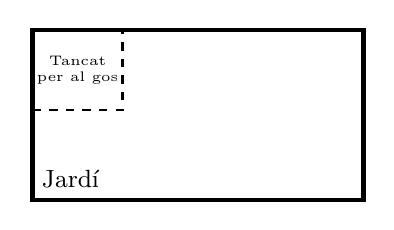
\begin{tikzpicture}[scale=0.6]
  \draw[line width=1.6pt] (0,0) rectangle (7,3.6);
  \draw[dashed,thick] (0,1.9) -- (1.9,1.9) -- (1.9,3.6);
  \node[font=\tiny,align=center] at (0.95,2.75) {Tancat\\per al gos};
  \node[font=\small] at (0.8,0.45) {Jardí};
\end{tikzpicture}
\end{center}
Ara podem reproduir els càlculs de l'apartat a) amb la nova situació. En aquest cas, el cost del tancat és
$C(x,y)=2{,}5\cdot(y+x)$ i, com que $y=\frac8x$, $C(x)=2{,}5\cdot\left(\frac8x+x\right)=2{,}5\cdot\left(\frac{8+x^2}{x}\right)$.
Calculant la primera derivada i igualant-la a 0:
\[
C'(x)=2{,}5\cdot\left(\frac{2x\cdot x-\left(8+x^2\right)\cdot1}{x^2}\right)=2{,}5\cdot\left(\frac{x^2-8}{x^2}\right)=0
\;\rightarrow\;x=\pm\sqrt8=\pm2\sqrt2\approx\pm2{,}83 .
\]
Anàlogament, l'única solució que té sentit és la positiva. Per comprovar si en $x=2\sqrt2$ hi ha un mínim, calculem la
segona derivada i n'observem el signe:
\[
C''(x)=2{,}5\cdot\left(\frac{2x\cdot x^2-\left(x^2-8\right)\cdot2x}{x^4}\right)
=2{,}5\cdot\left(\frac{2x^3-\left(2x^3-16x\right)}{x^4}\right)=2{,}5\cdot\frac{16}{x^3}.
\]
Com que $C''\!\left(2\sqrt2\right)>0$, en $x=2\sqrt2$ hi ha un mínim, i l'altura del tancat serà
$y=\frac{8}{2\sqrt2}=2\sqrt2$. Per tant, el tancat tindrà forma quadrada, de costat $2\sqrt2\approx2{,}83$ m. En aquest cas,
el preu mínim serà
\[
C\!\left(2\sqrt2\right)=2{,}5\cdot\left(\frac{8+\left(2\sqrt2\right)^2}{2\sqrt2}\right)=2{,}5\cdot\frac{16}{\sqrt8}=2{,}5\cdot2\sqrt8=14{,}14\ \text{€},
\]
i tindríem un estalvi de $20-14{,}14=\boxed{5{,}86\ \text{€}}$.

\textit{Pauta oficial:} 0,25 per situar el tancat correctament i per la funció cost, 0,25 per la derivada, el punt
singular i la justificació de mínim, i 0,25 per les dimensions i el càlcul de l'estalvi. Qualsevol altra argumentació
correcta serà considerada vàlida, encara que no es faci servir el càlcul diferencial, sempre que s'argumenti amb càlculs
matemàtics.
\end{solucio}

\end{apartats}
